We zeggen in de elektronica dat een stroom loopt van de + naar de -. In werkelijkheid bewegen de elektronen van de - naar de plus. Om stroom te laten lopen moet er een circuit\index{Circuit} zijn. Kortom de + moet op de \'e\'en of andere manier verbonden zijn met de -.

In de elektronica wordt een circuit schematisch weergeven met symbolen. Een voorbeeld zie je weergegeven in \ref{symbool:circuit}

\begin{figure}[h]
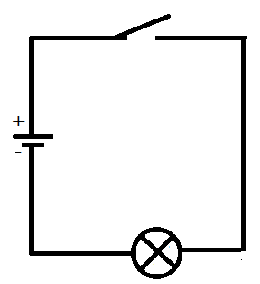
\includegraphics[width=5cm]{circuit}
\centering
\caption{Een circuit}
\label{symbool:circuit}
\end{figure}

